\begin{frame}[fragile] 
\secframetitle{\ssApproach}
\framesubtitle{\enzopcello\ approach}
%\framesubtitle{Scaling issues}
\begin{minipage}{3.0in}
%  AMR data structure scalability
%  Code development and maintenance
%  Ghost zone memory requirement
%  Patch size variation
%  Time stepping
%  Dynamic load balancing
%  Particle positions
%  Mesh quality
\begin{itemize}
\item \bfat{2}{\textcolor{red!50!black}{Memory usage}}
\begin{itemize}
  \item<2-> \textcolor{red}{AMR structure is fully distributed}
  \item<2-> \textcolor{red}{uniform blocks reduce fragmentation}
  \item<2-> \textcolor{red}{ghost zones allocated when needed$^*$}
\end{itemize}
\item \bfat{3}{\textcolor{green!50!black}{Mesh quality}}
\begin{itemize}
   \item<3-> \textcolor{green!80!black}{2-to-1 refinement constraint maintained}
\end{itemize}
\item \bfat{4}{\textcolor{blue!50!black}{Parallel task definition}}
\begin{itemize}
   \item<4-> \textcolor{blue}{uniform field array sizes in blocks}
   \item<4-> \textcolor{blue}{sizes determined by user}
\end{itemize}
\item \bfat{5}{\textcolor{cyan!50!black}{Parallel task scheduling}}
\begin{itemize}
   \item<5-> \textcolor{cyan!80!black}{asynchronous, data-driven}
   \item<5-> \textcolor{cyan!80!black}{block-local time stepping$^*$}
\end{itemize}
\item \bfat{6}{\textcolor{orange!50!black}{Data locality}}
\begin{itemize}
   \item<6-> \textcolor{orange!80!black}{only nearest-neighbor communication}
\end{itemize}
\end{itemize}
\vspace{-0.1in}
\only<1>{\textcolor{white}{\footnotesize $^*$ not implemented yet}}
\only<2-4>{\textcolor{red}{\footnotesize $^*$ not implemented yet}}
\only<5-6>{\textcolor{cyan!80!black}{\footnotesize $^*$ not implemented yet}}
\end{minipage} \
\begin{minipage}{1.0in}
\vspace{-0.2in}
\centerline{\tiny{Enzo}} 
\vspace{0.1in}
\centerline{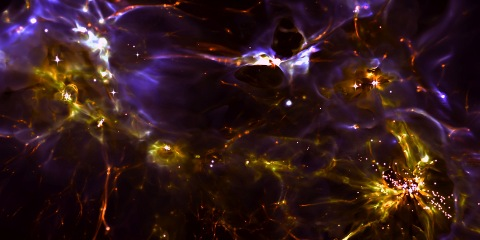
\includegraphics[width=2.0in,angle=90]{jhw-dwarf-galaxies.jpg}}
\centerline{\tiny{[ John Wise ]}}
\end{minipage}
\end{frame}
